\section{\label{sec:phases}Phase Transitions and Order Parameters}

The microscopic realization of a crystal reveals a lattice of ordered atoms. The lattice has a large $N$ number of atoms arranged in an ordered manner, with translational and rotational symmetry. To classify and explain the properties of materials, many theories were proposed. The \textit{principle of emergence} motivated the development of phenomenological methods to explain the properties of matter, which are based on a local \textit{order parameter} such as the magnetization $M$ for ferromagnetic phase transition as opposed to microscopic features such as spins, atoms, and molecules. These \textit{order parameters} characterize the organization of microscopic particles in the system, and are functions of coarse-grained variables such as temperatures and pressure. In his development of a theory of phase transition, Landau and Ginzburg \cite{hohenberg_introduction_2015,ter_haar_29_1965, wen_colloquium_2017} successfully associated different orders and hence different phases of materials, to different symmetries. He proposed that a discontinuity of the order parameter would cause a change of phase (or a phase transition), by spontaneously breaking the symmetry of the material. 

\begin{figure}[thpb] %this figure will be at the right
    \centering
    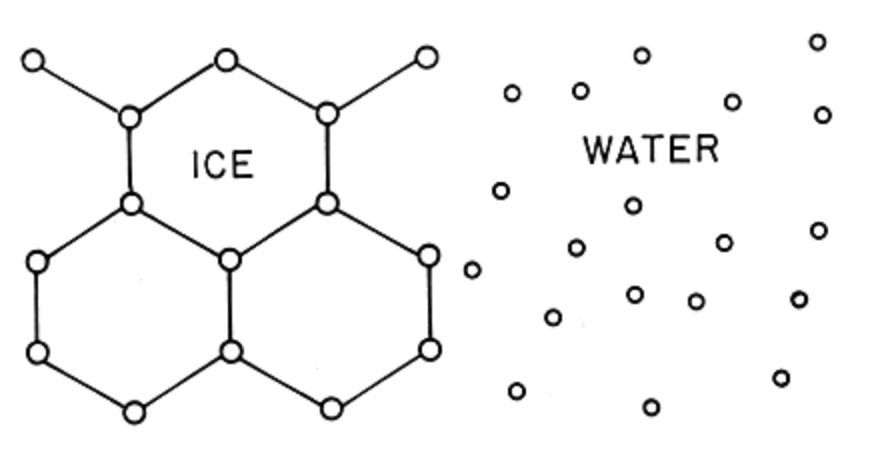
\includegraphics[width=0.25\textwidth]{figs/water-vs-ice.png}
    \caption{\label{fig:water-vs-ice}Ice breaks translational and rotational symmetries of water.}
\end{figure}

Crystals can be classified according to what types of symmetries are broken by their lattices. Crystals break translational and rotational symmetries of free space (e.g water losing translational and rotational symmetry by transition into ice). Liquid crystals only break the rotational symmetries. Magnets break time-reversal symmetry and the rotational symmetry of spin space. Superfluids (e.g low temperature $^{4}He$ at low temperature) break the $U(1)$ symmetry associated with the conservation of particles. 